\documentclass{article}
\usepackage[utf8]{inputenc}
\usepackage[T1]{fontenc}
\usepackage{graphicx}
\usepackage{hyperref}
\usepackage{geometry}
\geometry{margin=1in}

\title{MAGNETISM}
\date{Encyclopaedia Britannica (1771)}

\begin{document}
\maketitle

\section*{Historical source}
\textbf{Entry ID:} \texttt{entry-magnetism-756} \\
\textbf{Volume ID:} 191253808 \\
\textbf{Character Count:} 6815

\subsection*{Extracted Text}
But any degree of temper that is given to feed makes
a very important change in this respect. In the first
place, it acquires magnentifin more flowly by induction
than an equal and similar piece of common iron, and its
maly acquired lets. These differences are only trans-
mined by the deviations which it causes in the manner’s
needle from the magnetic meridian, and by its attractive
tions.

41 tempered
sheet
from a
the magma
film.

When the inducing magnet is removed, fome mag-
netti remains in the fixed bar, which retains the polo-
ry which, it will be the neighborhood of the matter.

Steel tempered to the degree fit for watch Springs
acquires along magnetic which is exhibits imme
disels on the removal of the magnet. But it diffipates
very fat ; and, in a very few minutes, it is reduced to
lois than one half of its strength while in control with
the magnet, and not two thirds of what it was
distety on removal from it. It continues to diffidate for
former days, though the her be kept with care'; but the
diffusion diminishes at, and in the near at, half over
third of its greatest power forany length of time, unleef
cardially keep or indjudicially treated.

Steel tempered into flowing cutting tools, fish a schlieb,
punches, and drills for metal, acquires magnifin fill
more flowly by induction, and acquires five of it while
in contact with the magnet, but it certain it more firms
by, and finally retains a greater proportion of who it
had acquired.

Steel made as hard as possible, is much longer in ac-
quiring all the magnifin which limple juxtaposition
can give to it. It acquires less than the formerly but it
retains is with great firmness, and finally retains a much
greater proportion.

Such one of iron as are fulcypible of magnetifi,
are nearly like hard feel in their effects you that in
the time necessary for their \_properlift\_ impregnation, and
in the durability of the acquired magnifine. They
effic exceedingly in respect to the degree of power
which they can attain by mere juxtaption, and the
virieties form to depend on heterogeneous mixture.
We emit offriever, thus far once of our ones of influence of
of magnetism of the metal in the fate of my way, and com-
bred with dolphins, are not magnentable while remain-
ing in that there. Mott core require reading, and a fort
of cementation, in contact with inflammable fuhlances.
This matter is not underdefended, but it would form
that complex metallization is far from being the north to
votrale condition, and that a certain degree of oxyda-
tion, and perhaps some other positive yet unknown,
make the her lautiness. Our all this is extremely
oblicure. The late Dr Cowin Knight made a compolio-
tion which required every phono and permanent mag-
seting, but the recent died with him. Dr Gilbert
peaks of limilat compositions, in which ferruginous
days were ingredients ; but we know nothing of the fate
of the metal in them, nor their mode of acquiring mag-
retin.

It is of peculiar importance to work that the ac-
quition of magnetization is gradual and progrestive, and
that the gradation is the more perceptible in proportion
as the field is of a hastheric temper. When a magnet is
hrough to one end of a bar of common iron, to remote
extremity, unleef exceedingly long, requires its utmost
magnifin immediately. But when the north pole of

Surez, Vol. II. Part I.

a magnet is applied: to one end of a bar of hard flee,
the part in contact immediately becomes a fourth pole,
and the far end is not yet affected. We offer a north
pole formed a fance difference from the concept, and bec-
sent that a faint tooth pole. "Their gradually advance
along the bar. The remote extremity become frit a
faint fourth pole, and it is not differ very long while
(If ceer) that it becomes a simple, vigorous, north
pole. More frequently it remains a difficult and recycle
north pole: may, if the her for very long, it often hop-
pus that have a sacrifice of north and forth poles,
which never make their way to the far end of the bar.
This phenomenon was first observed (we think) by Dr
Brook Taylor, who \_they\_ now account of his obtivations
to the \_Philophysical Transformation\_, no 344.

From the account we have given of their phenomenons to a st-
of indeed magnifine, it appears that the temporary because
magnifin is always lo disfpided that the rim of their beces
mutual attractions of the difficiliate poles exceeds the
gentich
im of the repollon between the limlar, poles, and
that therefore the two magnets tend to each other.
This is evidently equivalent to flying, that a piece of
magnungtic iron is always attracted by a magnet. No
exception has ever been observed to this fact, for Phys's
dury of a Thamades, or loadlines, which repeals iron, is
allowed by all to have been a false.

We think outfellow authorified to lay that this attraction
of the headlines for iron, or this tendency of iron
to the headline, is a secondary phenomenon, and is the
\_conference\_ of the proper disposition of the induced mag-
netimin. The proofs already given of the compound
matters of this phenomena, namely, that is arise from
the excess of two attributions above two repetitions, need
(we imagine) no addition. But the following condir-
actions place the matter beyond doubt.

I. The magnifinal of the two poles is evidently of an
opposite nature; the one repelling what the other at-
trade). If the aircraft iron, therefore, the other
should result it. But each path, by changing a magre-
tifion opposite to its own, on the nearest end of the iron,
and the fans with its own on the remote end, and its
action diminishing with an increase of diflants, there
mult always be an excess of attraction, and the iron mult
be attached.

A Each of the magnets A and B, in either of the
positions reprefened in fig. 12. would alone attract the
piece of common iron. But when placed together,
the fourth pole of 8 tends to render the upper end of
C a north pole; while the north pole of B tends to
take it a South pole. If there actions be nearly equal,
the weight of C cannot be supposedly be the magnifin
induced by any difference of action that may remain.
While C is hanging D I alone, let. A be gradually
enough tree, it gradually thorley the action of the
north pole of B, to that C gradually lofos its magnifin
and polarity, and its weight prends.

§. He all three cases where the induction of magne-
tifism is flow, the attraction is weak in proportion. This
is particularly remarked by Dr Gilbers. If we take
piece of common iron, and of fleet of different temps,
but all of the fame fine and form, we shall find that the
iron is much more thought attracted than any of the
rel, and that the attraction for each of them a weaker
proportion as they are harder. This liberty is to
accurately observed, that when the piece is thoroughly

R

\subsection*{Matched Wikipedia Article}
\textbf{Title:} Magnet \\
\textbf{Page ID:} 51079 \\
\textbf{Revision ID:} 1352951244 \\
\textbf{URL:} \url{https://en.wikipedia.org/wiki/Magnet}


\section*{Source record}
\begin{itemize}
\item \textbf{Dataset:} \texttt{NationalLibraryOfScotland/encyclopaedia\_britannica\_illustrated}
\item \textbf{Dataset Revision:} \texttt{309f765b1ecc83e0a7f7762e44b4a927a7555443}
\item \textbf{Page ID:} \texttt{britannica:309f765b1ecc83e0a7f7762e44b4a927a7555443:train:756} \\
  \textbf{Filename:} \texttt{page-0756-33eb91fcbe8d.jpg} \\
  \textbf{Row Index:} 756 \\
  \textbf{SHA256:} \texttt{33eb91fcbe8d9d08...}
\end{itemize}

\begin{figure}[h]
\centering
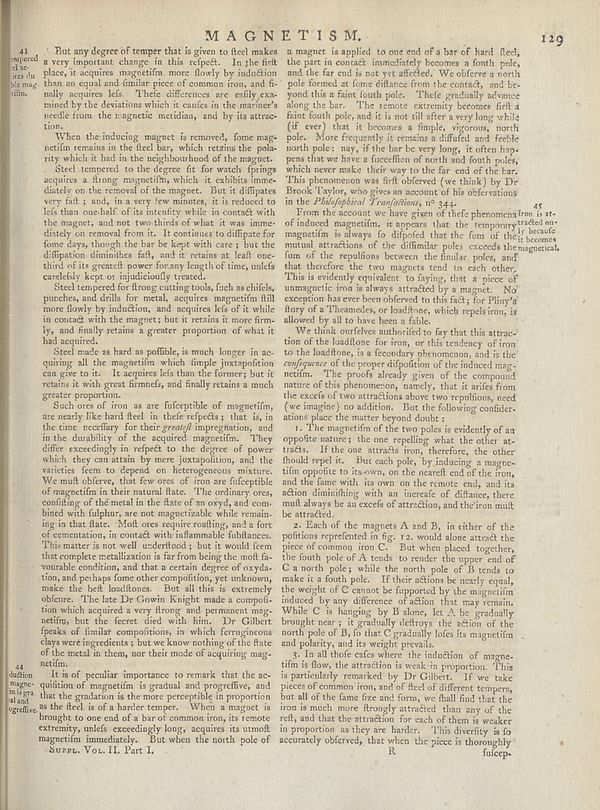
\includegraphics[width=0.85\textwidth]{../scans/page-0756-33eb91fcbe8d.jpg}
\caption*{Source scan: \texttt{page-0756-33eb91fcbe8d.jpg}}
\end{figure}

\end{document}
